% zip ms_files.zip ms.tex abstract.tex intro.tex method.tex results.tex conclusion.tex Praesepe.pdf variance.pdf simulated_CMD.pdf rotation_model_praesepe.pdf simulation_results.pdf NGC6819.pdf NGC6819_results.pdf hz.bib

\documentclass[useAMS, usenatbib, preprint, 12pt]{aastex}
% \documentclass[a4paper,fleqn,usenatbib,useAMS]{mnras}
\usepackage{cite, natbib}
\usepackage{float}
\usepackage{amsmath}
\usepackage{hyperref}
\usepackage{epsfig}
\usepackage{cases}
\usepackage[section]{placeins}
\usepackage{graphicx, subfigure}
\usepackage{color}
\usepackage{bm}

\AtBeginDocument{\let\textlabel\label}

\newcommand{\ie}{{\it i.e.}}
\newcommand{\eg}{{\it e.g.}}
\newcommand{\etal}{{\it et al.}}

\newcommand{\kepler}{{\it Kepler}}
\newcommand{\Kepler}{{\it Kepler}}
\newcommand{\corot}{{\it CoRoT}}
\newcommand{\Ktwo}{{\it K2}}
\newcommand{\ktwo}{\Ktwo}
\newcommand{\TESS}{{\it TESS}}
\newcommand{\tess}{{\it TESS}}
\newcommand{\LSST}{{\it LSST}}
\newcommand{\lsst}{{\it LSST}}
\newcommand{\Wfirst}{{\it WFIRST}}
\newcommand{\wfirst}{{\it WFIRST}}
\newcommand{\SDSS}{{\it SDSS}}
\newcommand{\PLATO}{{\it PLATO}}
\newcommand{\plato}{{\it PLATO}}
\newcommand{\Gaia}{{\it Gaia}}
\newcommand{\gaia}{{\it Gaia}}
\newcommand{\panstarrs}{{\it PanSTARRS}}

\newcommand{\Teff}{$T_{\mathrm{eff}}$}
\newcommand{\teff}{$T_{\mathrm{eff}}$}
\newcommand{\FeH}{[Fe/H]}
\newcommand{\feh}{[Fe/H]}
\newcommand{\prot}{$P_{\mathrm{rot}}$}
\newcommand{\pmega}{$\bar{\omega}$}
\newcommand{\mj}{$m_j$}
\newcommand{\mh}{$m_h$}
\newcommand{\mk}{$m_k$}
\newcommand{\mx}{$m_x$}
\newcommand{\logg}{log(g)}
\newcommand{\dnu}{$\Delta \nu$}
\newcommand{\numax}{$\nu_{\mathrm{max}}$}
\newcommand{\degrees}{$^\circ$}
\newcommand{\vz}{$v_z$}
\newcommand{\vb}{$v_b$}
\newcommand{\kms}{$kms^{-1}$}

% \newcommand{\nsim_stars}{841}

\newcommand{\amnh}{1}
\newcommand{\cca}{2}
\newcommand{\hawaii}{3}

\newcommand{\sd}{{\tt stardate}}
\newcommand{\gcolor}{$G_{BP} - G_{RP}$}
\newcommand{\mcp}{\citep{mcquillan2014}}
\newcommand{\mct}{\citet{mcquillan2014}}
\newcommand{\bvector}{${\bf b}$}
\newcommand{\python}{{\it Python}}

\newcommand{\racomment}[1]{{\color{blue}#1}}

\begin{document}

\title{Exploring the ages of rotating stars using galactic dynamics: a novel
approach to calibrating gyrochronology}

\author{%
    Ruth Angus,
    Angus Beane,
    Adrian Price-Whelan,
    Jennifer van Saders,
    Elisabeth Newton,
    Travis Berger,
    Dan Foreman-Mackey,
    Lauren Anderson,
    Megan Bedell,
    Jackie Faherty,
    Rocio Kiman,
    Melissa Ness}

% \altaffiltext{\amnh}{American Museum of Natural History, Central Park West,
% Manhattan, NY, USA}
% \altaffiltext{\cca}{Center for Computational Astrophysics, Flatiron Institute,
% 162 5th Avenue, Manhattan, NY, USA}
% \altaffiltext{\hawaii}{Institute for Astronomy, University of Hawai'i at
% M\={a}noa, Honolulu, HI, USA}

% Still to do: deredden before calculating ages.

% Word limit: 3500

% Word limit: 250, currently 230
\begin{abstract}
    % The distribution of rotation periods of K and M stars, measured from light
% curves obtained from the \kepler\ spacecraft, has a sharp mass-dependent gap
% at around 10-20 days.
% This gap traces a line of constant age and constant Rossby number in the
% rotation period-effective temperature plane, indicating that the cause could
% be related to a discontinuity in either the local star formation history, or
% the magnetic braking evolution of stars.
% A third explanation for the rotation period gap is measurement error caused by
% confounders such as binary companions or aliasing.
% For example, the lower rotation sequence could be a reflection of the upper
% sequence, caused by incorrect measurements at half the true period.
% In this paper, we rule out the possibility that this gap could be caused by
% incorrect period measurements or binary companions, by showing that the
% rapidly rotating stars are dynamically young.

% We also find that nai/"vely applying gyrochronology relations to stars hotter
% than around 5000 K can result in inaccurate ages.

% Finally, we show that the changing shape of the rotation-temperature relations
% causes the `M dwarf dip', providing further evidence that the gyrochronology
% relations are not separable functions of color and age.

The rotational evolution of FGKM dwarfs is still mostly unconstrained after
around 2-3 billion years.
This limit is set by the oldest open clusters whose members have precise light
curves, and therefore photometric rotation periods.
However, recent evidence suggests that the relationship between rotation
period and color/temperature/mass does not remain constant over large
timescales, as has long been assumed.
Old clusters seem to have a flatter relationship between rotation period and
color than young clusters.
In addition, old field stars with asteroseismic ages, observed by the \kepler\
spacecraft, appear to be rotating more rapidly than expected for their ages
and masses.
In this work we use the velocity dispersion of groups of stars as a proxy for
age in order to demonstrate that the relationship between rotation period and
effective temperature not only changes over time but even appears to invert.
At young ages G stars rotate more rapidly than K and M dwarfs, but at old ages
they appear to rotate more rapidly.
In addition, we show that stars rotating just below the rotation period gap
are dynamically young, we ruling out the possibility that the rotation period
gap is caused by incorrect period measurements or binary companions.

\end{abstract}

% Word limit: 750, currently: 674.
% Word limit: 500
\section{Introduction}

\subsection{Gyrochronology}

Stars with significant convective envelopes ($\lesssim$ 1.3 M$_\odot$) have
strong magnetic fields and spin more slowly over time through magnetic braking
\citep[\eg][]{schatzman1962, weber1967, skumanich1972, kawaler1988,
pinsonneault1989}.
Although stars are typically born with random rotation periods, ranging from 1
to 10 days, observations of young open clusters reveal that their rotation
periods converge onto a unique sequence by $\sim$500-700 million years
\citep[\eg][]{irwin2009}.
After this time, it is thought that the rotation period of a star is
determined, to first order, by its color and age alone.
This is the principle behind gyrochronology -- the method of inferring a
star’s age from its rotation period \citep[\eg][]{barnes2003, barnes2007,
barnes2010, meibom2011, meibom2015}.
% It is well established that magnetized stellar winds cause the rotation
% periods of FGKM dwarfs to increase over time \citep[\eg][]{schatzman1962,
% weber1967, skumanich1972, kawaler1988, pinsonneault1989}, and, once fully
% calibrated, the relationship between period, mass and age can be used to
% age-date stars via gyrochronology \citep{barnes2003, barnes2007, barnes2010,
% meibom2011, meibom2015}.
However, new photometric rotation periods made available by the \kepler\
\citep{borucki2010} and \ktwo\ \citep{howell2014} missions
\citep[\eg][]{mcquillan2014, garcia2014, douglas2017, rebull2017, meibom2011,
meibom2015, curtis2019} reveal that rotational evolution is more complicated
than previously thought.
For example, the M dwarfs in the $\sim$ 650 Myr Praesepe cluster spin more
slowly than the G dwarfs -- in theory because lower-mass stars have deeper
convections zones which generate stronger magnetic fields and more efficient
magnetic braking.
However, in the 1.1 Gyr NGC 6811 cluster, late-K dwarfs rotate at the {\it
same} rate as early-K dwarfs \citep{curtis2019}.
In other words, convection zone depth cannot be the only variable that affects
stellar spin-down rate.
New semi-empirical models that vary the rate of angular momentum
redistribution in the interiors of stars are able to reproduce this flattened
period-color relation \citep{spada2019}.
These models suggest that mass and age-dependent angular momentum transport
between the cores and envelopes of stars has a significant impact on their
surface rotation rates.

Another example of unexpected rotational evolution is seen in old field stars
which appear to rotate more rapidly than classical gyrochronology models
predict \citep{angus2015, vansaders2016, vansaders2018, metcalfe2019}.
A mass-dependent modification to the classical \prot\ $\propto
t^{\frac{1}{2}}$ spin-down law \citep{skumanich1972} is required to reproduce
these observations.
To fit magnetic braking models to these data, a cessation of magnetic braking
is required after stars reach a Rossby number (ratio of rotation period to
convective turnover time) of around 2 \citep{vansaders2016, vansaders2018}.

The rotational evolution of stars is clearly a complicated process, and to
fully calibrate the gyrochronology relations we need reliable ages for large
numbers of field stars which span a range of ages.
% however relying on open clusters (which are typically young) and asteroseismic
% stars (which are typically G-type stars or more massive) to calibrate
% gyrochronology relations limits the mass and age coverage of the calibration
% sample.
In this paper, we use the velocity dispersions of field stars to gain insight
into their rotational evolution.
Velocity dispersion provides relative ages for groups of stars, allowing us to
observe the rotational evolution of stars over a range of masses and ages.

\subsection{Using kinematics as an age proxy}

Stars are thought to be born in the thin disk of the Milky Way (MW), orbiting
the galaxy with a low out-of-plane, or vertical, velocity ($W$, or \vz),
just like the star-forming molecular gas observed in the disk today
\citep[\eg][]{stark1989, stark2005, aumer2009, martig2014, aumer2016}.
On average, the vertical velocities of stars increase over time
\citep[\eg][]{nordstrom2004, holmberg2007, holmberg2009, aumer2009,
casagrande2011}.
Although the cause of dynamical heating is not well understood, interactions
with giant molecular clouds, spiral arms and the galactic bar are thought to
play an important role \citep[see][for a review of secular evolution in the
MW]{sellwood2014}.
Although the velocity of any individual star will only provide a weak age
constraint, the velocity {\it dispersion} of a {\it group} of stars can
indicate whether, on average, that group is old or young relative to other
groups.
In this work we compare the velocity dispersions of groups of field stars in
the Galactic thin disk to ascertain which groups are older and which younger
and draw conclusions based on the implied relative ages.
% The age-velocity dispersion reations (AVRs) are still actively being

% Vertical action is thought to be a better age indicator than vertical
% velocity \citep{ting2019}, although still only a weak age indicator for
% individual stars \citep{beane2018}, however both vertical action ($J_z$) and
% vertical
Vertical velocity, \vz, can only be calculated with full 6-dimensional
position and velocity information, and unfortunately most stars with measured
rotation periods do not have radial velocity (RV) measurements because they
are relatively faint \kepler\ targets ($\sim$11th-18th magnitudes).
For this reason, we used velocity in the direction of galactic latitude, \vb,
to approximate \vz.
The \kepler\ field is positioned at low galactic latitude
(b=$\sim$5-20\degrees), so \vb\ is a close (although imperfect -- see section
\ref{sec:results}) approximation to \vz.
Because we use \vb\ rather than \vz\, we cannot calculate absolute kinematic
ages using an age-velocity dispersion relation (AVR).
However, regardless of direction, velocity dispersion is expected to
monotonically increase over time, and can therefore be used to {\it rank}
groups of stars by age.

This paper is laid out as follows: in section \ref{sec:method} we describe our
sample selection process and the methods used to calculated stellar
velocities.
We also establish that \vb\ velocity dispersion, \sigmavb, can be used as an
age proxy by demonstrating that neither mass-dependent heating nor the
selection function seems to strongly affect on our sample.
In section \ref{sec:results} we use kinematics to investigate the
relationship between rotation period, age and color/\teff\ in the field and
interpret our results in section \ref{sec:discussion}.
% We show that the period-color relation of Praesepe is not applicable to
% old stars in section \ref{sec:age_cut}, and reveal the true shape of the
% period-color relations in section \ref{sec:the_reveal}.
% We discuss a possible connection with the rotation period gap in section
% \ref{sec:period_gap}.

% We also tested the \citet{angus2019} gyrochronology relation, a separable
% relation in color and age, calibrated using the period-color relation of
% Praesepe (in \gaia\ \gcolor\ color) and the period-age relation of Praesepe
% and the Sun.
% The large number of Praesepe members with precise rotation periods from the
% \ktwo\ mission \citep{douglas2017, rebull2017}, spanning spectral types F
% through early M, makes it a good cluster for calibrating the period-color
% relation of stars at 650 Myrs.
% However, although this relation accurately describes the rotation periods of F
% and G stars up to around 2.5 Gyr (the age of NGC 6819 -- the oldest cluster
% with available rotation periods), it over-predicts the rotation periods of K
% dwarfs in the 1.1 Gyr NGC 6811 cluster.
% Very few reliable age estimates exist for K dwarfs with rotation periods older
% than 1.1 Gyr, or between the ages of $\sim$ 800 Myr--1.1 Gyr so the rotational
% evolution of middle-aged K dwarfs is largely unknown.
% The oldest M dwarfs with reliable ages and rotation periods are members of
% Praesepe ($\sim$ 650 Myrs), so even {\it less} is known about their rotational
% evolution.

% We calculated gyrochronal ages of cool field dwarfs in the \kepler\ field
% using the \citep{angus2019} gyrochronology model, with de-reddened \Gaia\
% \gcolor\ color and rotation periods reported by \mct\ (we explain our data
% selection process in section \ref{sec:the_data}).
% These gyrochronal ages are shown on a \gaia\ color-magnitude diagram (CMD) in
% figure \ref{fig:age_gradient}.
% The stars with old gyrochronal ages, plotted in yellow hues, predominantly lie
% along the upper edge of the MS, where stellar evolution models predict old
% stars to be, however the majority of these `old' stars are bluer than \gcolor\
% $\sim$ 1.5 dex.
% This suggests that the \citet{angus2019} gyrochronology relation
% under-predicts the ages of low-mass stars.
% There is no reason to expect the oldest stars in this sample to be the bluer
% ones: M dwarfs are, on average, older than K dwarfs and are expected to remain
% active for longer, so should therefore have measurable rotation periods at
% older ages.
% Since the \citet{angus2019} gyrochronology model, which is based on the
% period-color relation of Praesepe, predicts the oldest stars in this sample to
% be K dwarfs, it is probably either under-predicting M dwarf ages or
% over-predicting K dwarf ages.
% % In other words, old M dwarfs rotate more rapidly or K dwarfs rotate more
% % slowly than the model predicts.
% In what follows, we use a population-based stellar age indicator, velocity
% dispersion, to investigate the gyrochronology relations at old ages in
% the field.


% Word limit: 500, currently 336.
\section{Method}
\label{sec:method}

\subsection{The data}
\label{sec:the_data}

We used the publicly available \kepler-\gaia\ DR2 crossmatched
catalog\footnote{Available at gaia-kepler.fun} to combine the \mct\ catalog of
stellar rotation periods, measured from \kepler\ light curves, with the \gaia\
DR2 catalog of parallaxes, proper motions and apparent magnitudes.
Reddening and extinction from dust was calculated for each star using the
Bayestar dust map implemented in the {\tt dustmaps} {\it Python} package
\citep{green2018}, and {\tt astropy} \citep{astropy2013, astropy2018}.

For this work, we used the precise \textit{Gaia} DR2 photometric color,
$G_{\rm BP} - G_{\rm RP}$, to estimate \teff\ for the Kepler rotators.
Curtis \etal\ (2020, in prep) combined effective temperature measurements for
nearby, unreddened field stars in benchmark samples, including FGK stars
characterized with high-resolution optical spectroscopy \citep{brewer2016}, M
dwarfs characterized with low-resolution optical and near-infrared
spectroscopy \citep{mann2015}, and K and M dwarfs characterized with
interferometry and bolometric flux analyses \citep{boyajian2012}.
This empirical color--temperature relation is valid over the color range $0.55
< (G_{\rm BP} - G_{\rm RP})_0 < 3.20$, corresponding to $6470 < T_{\rm eff} <
3070$~K.
The dispersion about the relation implies a high precision of 50~K.
These benchmark data enable us to accurately estimate \teff\ for cool dwarfs
\citep[\eg][]{rabus2019}, and allows us to correct for interstellar reddening
at all temperatures\footnote{The color--temperature relation is described in
detail in the Appendix of, and the formula is provided in Table 4 of, Curtis
\etal\ (2020, in prep).}.
The equation we used to calculate photometric temperatures from Gaia \gcolor\
color is a seventh-order polynomial with coefficients given in table
\ref{tab:coeffs}.
\begin{table}[h!]
  \begin{center}
      \caption{
          Coefficient values for the 7th-order polynomial used to estimate
      \teff\ from \Gaia\ \gcolor\ color, calibrated in Curtis \etal\ (2020, in
      prep).}
    \label{tab:coeffs}
    \begin{tabular}{l|c} % <-- Alignments: 1st column left and 2nd middle, with vertical lines in between
        (\gcolor\ ) exponent & Coefficient  \\
      \hline
      $0$ & -416.585 \\
      $1$ & 39780.0  \\
      $2$ & -84190.5 \\
      $3$ & 85203.9  \\
      $4$ & -48225.9 \\
      $5$ & 15598.5  \\
      $6$ & -2694.76 \\
      $7$ & 192.865  \\
    \end{tabular}
  \end{center}
\end{table}

Photometric binaries and subgiants were removed from the \mct\ sample by
applying cuts to the color-magnitude diagram (CMD), shown in figure
\ref{fig:age_gradient}.
A 6th-order polynomial was fit to the main sequence and raised by 0.27 dex to
approximate the division between single stars and photometric binaries (shown
as the curved dashed line in figure \ref{fig:age_gradient}).
All stars above this line were removed from the sample.
Subgiants were also removed by eliminating stars brighter than 4th magnitude
in \gaia\ G-band.

The rotation periods of the dwarf stars in the \mct\ sample are shown on a
\gaia\ color-magnitude diagram (CMD) in the top panel of figure
\ref{fig:age_gradient}.
In the bottom panel, the stars are colored by their gyrochronal age,
calculated using the \citet{angus2019} gyrochronology relation.
The stars with old gyrochronal ages, plotted in purple hues, predominantly lie
along the upper edge of the MS, where stellar evolution models predict old
stars to be, however the majority of these `old' stars are bluer than \gcolor\
$\sim$ 1.5 dex.
The lack of gyrochronologically old M dwarfs suggests that either old M dwarfs
are missing from the \mct\ catalog, or the \citet{angus2019} gyrochronology
relation under-predicts the ages of low-mass stars.
Given that lower-mass stars stay active for longer than higher-mass stars
\citep[\eg][]{west2011, kiman2019}, and are therefore more likely to have
measurable rotation periods at old ages, the latter scenario seems likely.
However, it is also possible that the rotation periods of the oldest early M
dwarfs are so long that they are not measurable with Kepler data.
Ground-based rotation period measurements of mid and late M dwarfs indicate
that there is an upper limit to the rotation periods of {\it late} M dwarfs of
around 140 days \citep{newton2016, newton2017, newton2018}, which is much
longer than the longest rotation periods measured in the \mct\ sample (around
70 days).
The apparent lack of old ages for M dwarfs in figure \ref{fig:age_gradient}
may be caused by a combination of ages being underestimated by a poorly
calibrated model, and rotation period detection bias.
The \citet{angus2019} gyrochronology relation is a simple polynomial model,
fit to the period-color relation of Praesepe.
Inaccuracies are a typical feature of empirically calibrated gyrochronology
models: since there are no (or at least very few) old M dwarfs with rotation
periods, the models are poorly calibrated for these stars.
\begin{figure}
  \caption{
      Top: de-reddened MS \kepler\ stars with \mct\ rotation periods, plotted
    on a \gaia\ CMD.
    We removed photometric binaries and subgiants from the sample by excluding
    stars above the dashed lines.
    Bottom: a zoom-in of the top panel, with stars colored by their
    gyrochronal age \citep{angus2019}, instead of their rotation period.
    A general age gradient is visible across the main sequence.
    Since the \citet{angus2019} relation predicts that the oldest stars in
    the \mct\ sample are late-G and early-K dwarfs, it is probably
    under-predicting the ages of late-K and early-M dwarfs.
}
  \centering
    \includegraphics[width=1\textwidth]{CMD_cuts_double}
\label{fig:age_gradient}
\end{figure}

The {\tt Pyia} \citep{price-whelan_2018} and {\tt astropy} \citep{astropy2013,
astropy2018} {\it Python} packages were used to calculate velocities for the
\mct\ sample.
{\tt Pyia} calculates velocity samples from the full \gaia\ uncertainty
covariance matrix via Monte Carlo sampling, thereby accounting for the
covariances between \gaia\ positions, parallaxes and proper motions.
Stars with negative parallaxes, parallax signal-to-noise ratios less than 10,
stars fainter than 16th magnitude, stars with absolute \vb\ uncertainties
greater than 1 \kms\, and stars with galactic latitudes greater than
15\degrees\ (justification provided in the appendix) were removed from the
sample.
Finally, we removed stars with rotation periods shorter than the main
population of periods, since this area of the period-\teff\ diagram is
sparsely populated.
We removed these rapid rotators by cutting out stars with gyrochronal ages
less than 0.5 Gyr \citep[based on the][gyro-model]{angus2019}, because a 0.5
Gyr gyrochrone\footnote{A gyrochrone is a gyrochronological isochrone, or a
line of constant age in period-\teff, or period-color space.} traces the
bottom edge of the main population of rotation periods.
After these cuts, around 13,000 stars out of the original $\sim$34,000 were
included in the sample.


% Word limit: 500, currently 1609
\section{Results and Discussion}
\label{sec:results}

\subsection{The period-\teff\ relations, revealed}
\label{sec:the_reveal}

To explore the relationship between rotation period, effective temperature
(\teff ) and velocity dispersion, we calculated \sigmavb \footnote{\sigmavb
was calculated as 1.5$\times$ the median absolute deviation, to mitigate
sensitivity to outliers.} for groups of stars with similar rotation periods
and temperatures, and presumed similar age.
The top panel of figure \ref{fig:vplot} shows rotation period versus effective
temperature for the \mct\ sample, coloured by \sigmavb, where \sigmavb\ was
calculated for groups of stars over a grid in $\log_{10}$(period) and
temperature.
If we assume that mass dependent heating does not strongly affect this sample
and \vb\ at low galactic latitudes is an unbiased tracer of \vz, then \vb\
velocity dispersion can be interpreted as an age proxy, and stars plotted in a
similar color in figure \ref{fig:vplot} are similar ages.
We discuss this assumption further in the appendix.
\begin{figure}
  \caption{
    Top: Rotation period vs effective temperature for stars in the \mct\
    sample, colored by the velocity dispersions of stars calculated over a
    grid in $\log_{10}$(period) and \teff.
    Black lines show gyrochrones from a gyrochronology model that projects the
    rotation-color relation of
    Praesepe to longer rotation periods over time \citep{angus2019}.
    These gyrochrones do not appear to reflect the evolution of field stars at
    long rotation periods/old ages because they do not trace lines of constant
    velocity dispersion.
    Gyrochrones are plotted at 0.5, 1, 1.5, 2, 2.5, 4 and 4.57 Gyr in both top
    and bottom panels.
    Bottom: Same as top panel with rotation period vs {\it mass}
    \citep[from][]{berger2020}.
    White lines show gyrochrones from a model that includes mass and
    age-dependent angular momentum transport between the core and envelope
    \citep{spada2019}.
    Qualitatively, these gyrochrones reflect the evolution of field
    stars at long rotation periods/old ages: they trace lines of constant
    velocity dispersion by reproducing periods of `stalled' rotational
    evolution for K-dwarfs.
}
  \centering
    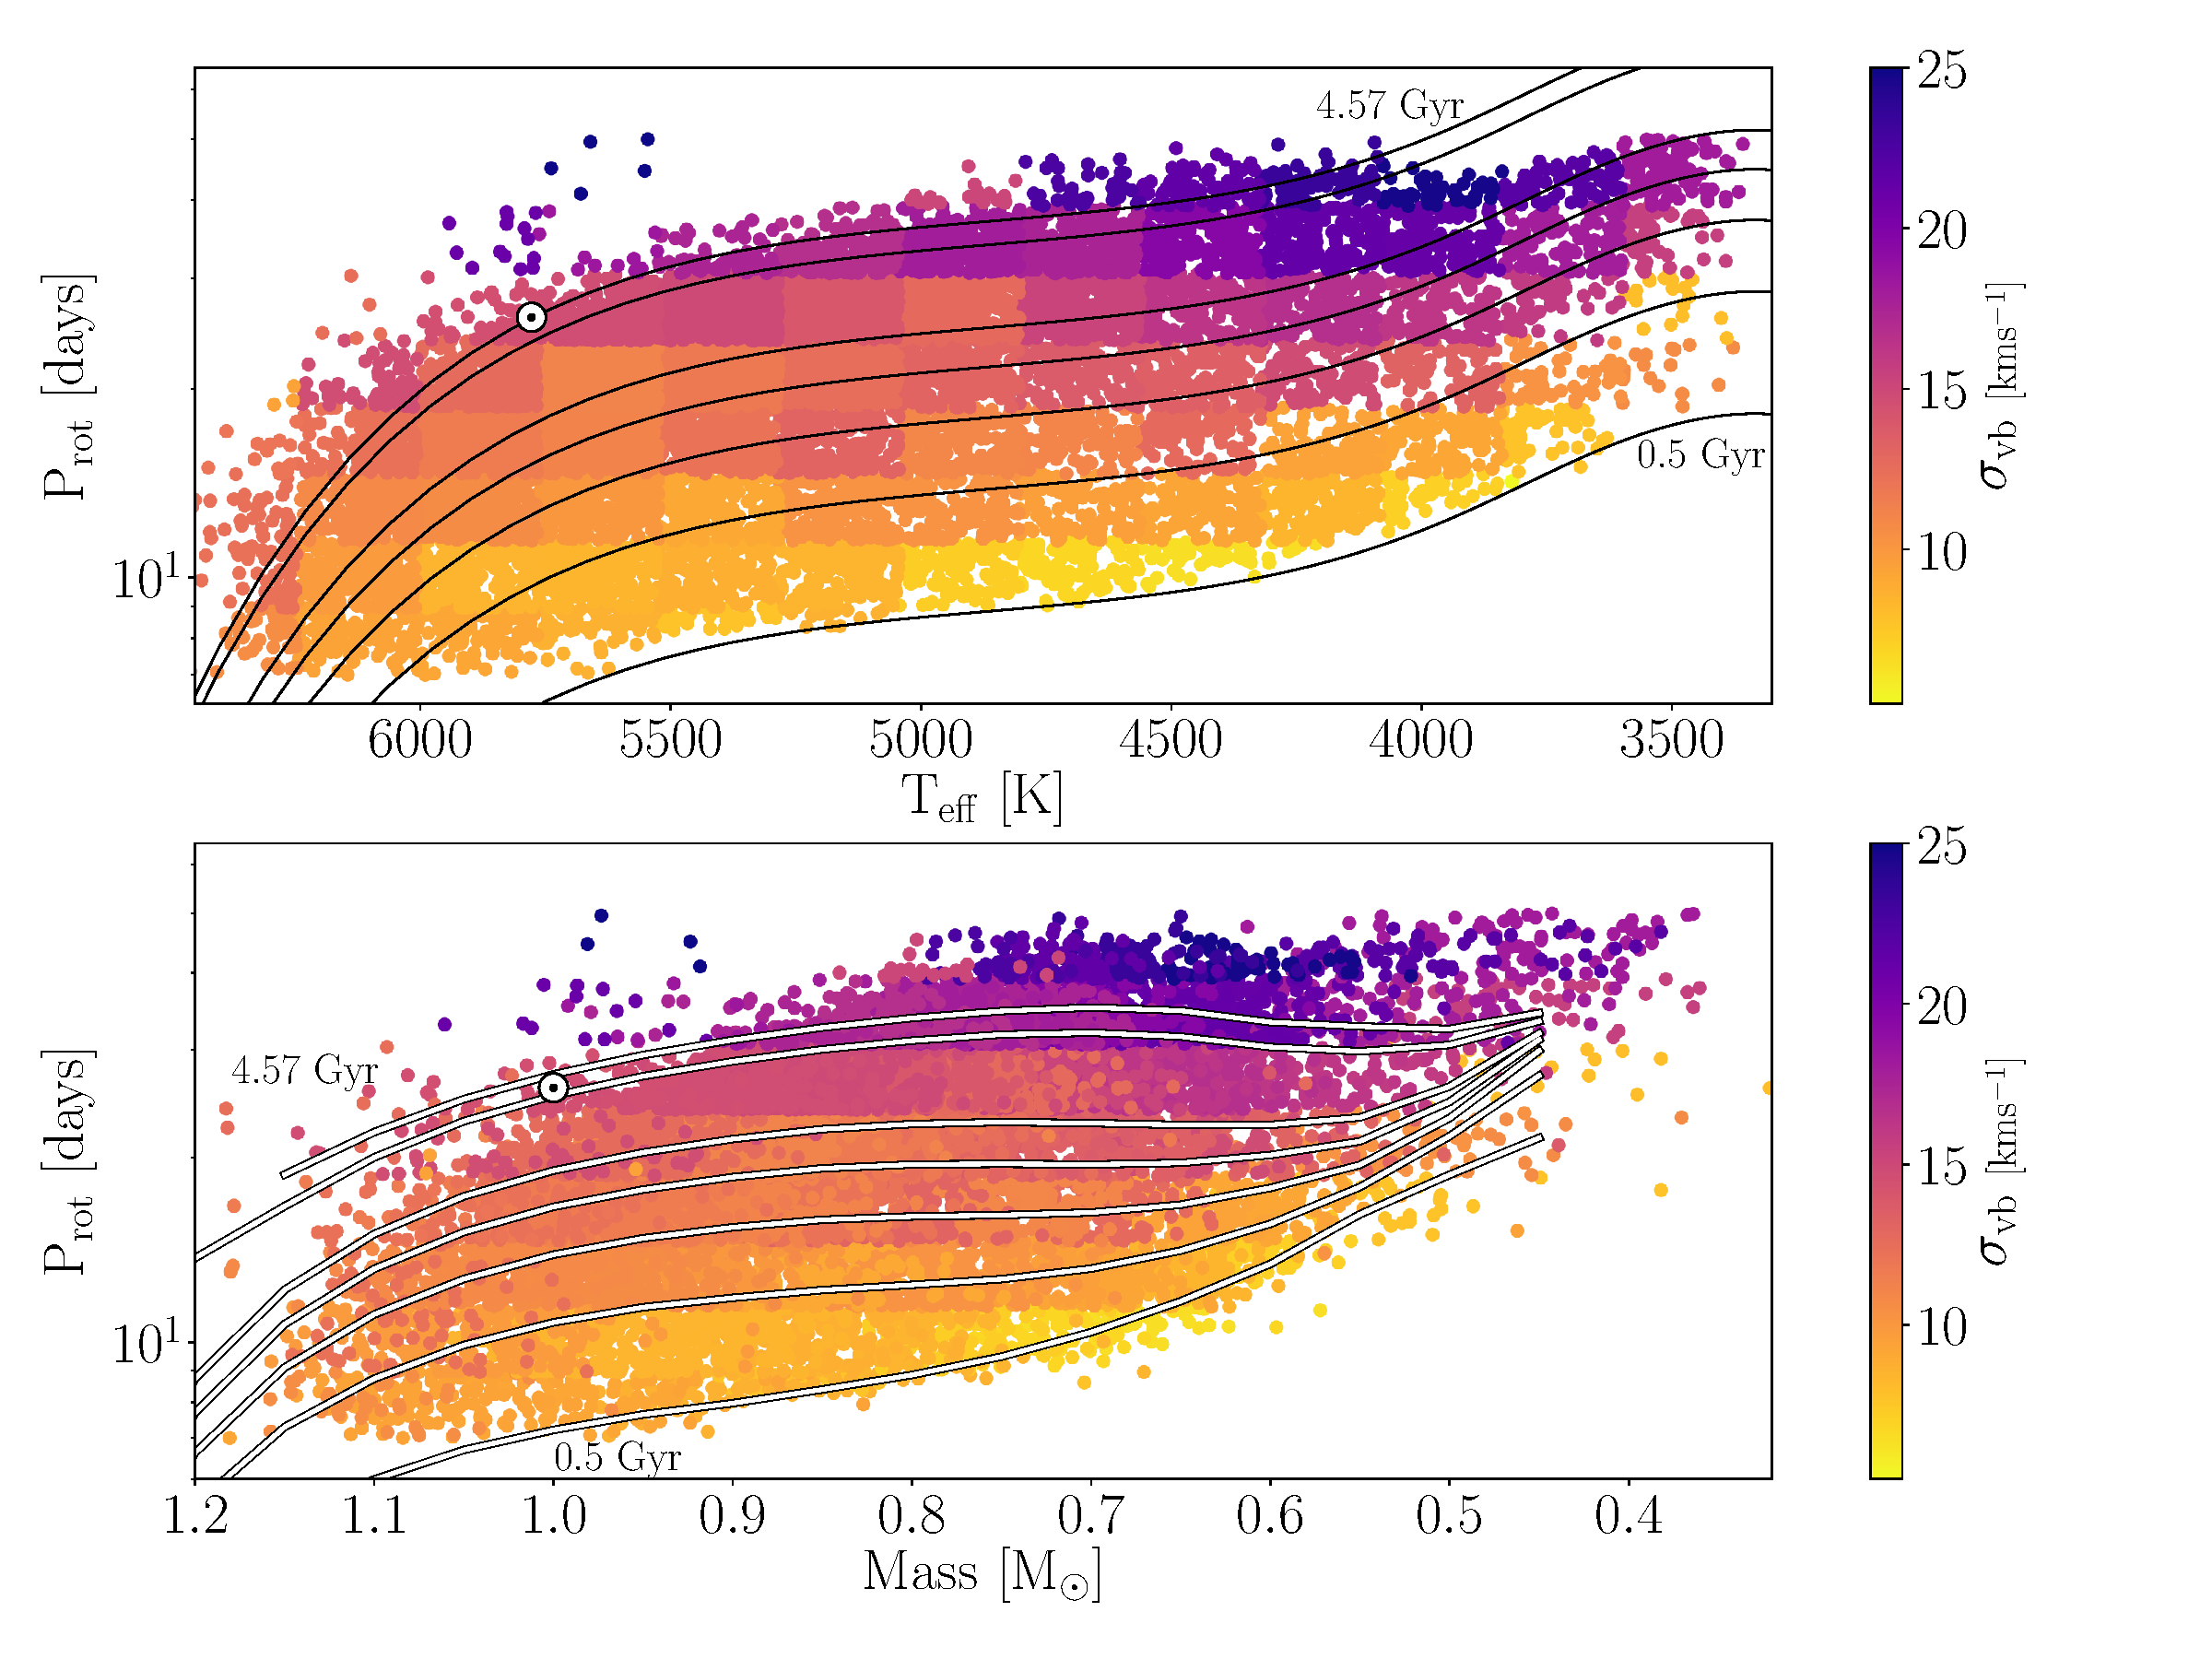
\includegraphics[width=1\textwidth]{main_figure}
\label{fig:vplot}
\end{figure}

Overall, figure \ref{fig:vplot} shows that velocity dispersion increases with
rotation period across all temperatures, implying that rotation period
increases with age, as expected.
This result is insensitive to the choice of bin position and size.
Black lines show gyrochrones from the \citet{angus2019} gyrochronology model,
which projects the rotation-color relation of Praesepe to longer rotation
periods over time.
These gyrochrones are plotted at 0.5, 1, 1.5, 2, 2.5, 4 and 4.57 Gyr.
At the youngest ages, these gyrochrones describe the data well: the palest
yellow (youngest) stars with the lowest velocity dispersions all fall close to
the 0.5 Gyr gyrochrone.
However, although the 0.5 Gyr and 1 Gyr gyrochrones also trace constant
velocity dispersion/age among the field stars, by 1.5 Gyr the gyrochrones
start to {\it cross} different velocity dispersion regimes.
For example, the 1.5 Gyr gyrochrone lies on top of stars with velocity
dispersions of around 10-11 kms$^{-1}$ at 5000-5500K and stars with $\sim$15
\kms\ velocity dispersions at 4000-4500K.
The gyrochrones older than 1.5 Gyr also cross a range of velocity dispersions.
If these were true isochrones they would follow lines of constant velocity
dispersion.
At ages older than around 1 Gyr, it appears that gyrochrones should have a
more flattened, or even inverted, shape in rotation period-\teff\ space than
these Praesepe-based models.

The bottom panel of figure \ref{fig:vplot} shows velocity dispersion as a
function of rotation period and {\it mass}, \citep[from][]{berger2020}, with
gyrochrones from the \citep{spada2019} model shown in white.
These gyrochrones are also plotted at 0.5, 1, 1.5, 2, 2.5, 4 and 4.57 Gyr.
Each point plotted in the top panel also appears in the bottom panel with the
same color.
Because velocity dispersion was calculated in bins of \teff, not mass, bin
outlines are clearly visible in the top panel but appear smeared-out in the
bottom panel.
In the bottom panel of figure \ref{fig:vplot}, the \citet{spada2019} models
{\it do} trace lines of constant velocity dispersion, and reproduce the trends
in the data at all ages.
These models qualitatively agree with the data and reproduce the apparent
flattening and inversion in the rotation period-\teff/mass relations.

The results shown in figure \ref{fig:vplot} indicate that stars of spectral
type ranging from late G to late K ($\sim$5500-3500 K) follow a braking law
that changes over time.
In particular, the relationship between rotation period and effective
temperature appears to flatten out and eventually invert.
These results provide further evidence for `stalled' rotational evolution of K
dwarfs, like that observed in open clusters \citep{curtis2019} and reproduced
by models that vary angular momentum transport between stellar core and
envelope with time and mass \citep{spada2019}.
The velocity dispersions of stars in the \mct\ sample provide the following
picture of rotational evolution.
At young ages \citep[younger than around 1 Gyr but still old enough to be on
the main sequence and have transitioned from the `I' sequence to the `C'
sequence ][]{barnes2003}, stellar rotation period {\it decreases} with {\it
increasing} mass.
This is likely because lower-mass stars with deeper convection zones have
stronger magnetic fields, larger Alfv\'en radii and therefore experience
greater angular momentum loss rate \citep[\eg][]{schatzman1962, parker1970,
kawaler1988, charbonneau2010}.
According to the \citet{spada2019} model, there is minimal transportation of
angular momentum from the surface to the core of the star at these young ages,
so the surface slows down but the core keeps spinning rapidly.
This aligns with the current assumptions about stellar spin-down, dynamo
theory, and the gyrochronology paradigm that has been in place for decades
\citep[\eg][]{skumanich1972, noyes1984, kawaler1988, barnes2003, angus2019}.
According to the data presented in figure \ref{fig:vplot} however, at
intermediate ages, the rotation periods of K dwarfs appear {\it constant} with
mass, and at late ages rotation period {\it increases} with {\it increaasing}
mass.
The interpretation of this, according to the \citet{spada2019} model, is that
lower-mass stars are still braking more efficiently at these intermediate and
old ages but their cores are more tightly coupled to their envelopes, allowing
angular momentum transport between the two layers.
Angular momentum resurfaces and prevents the stellar envelopes from
spinning-down rapidly, and this effect is strongest for late K-dwarfs with
effective temperatures of $\sim$4000-4500K and masses $\sim$0.5-0.7 M$_\odot$.

It has been demonstrated that lower-mass stars remain magnetically active
longer than more massive stars, \citep[\eg][]{west2008, kiman2019}.
If the detectability of a rotation period is considered to be a magnetic
activity proxy, then our results provide further evidence for a mass-dependent
activity lifetime.
Figure \ref{fig:vplot} shows that the groups of stars with the largest
velocity dispersions are cooler than 4500 K.
This implies that the oldest stars with detectable rotation periods, are
cooler than 4500 K, \ie\ these-low mass stars stay active longer than more
massive stars.
To investigate this idea further, we compared the velocity dispersions of
stars with measured rotation periods, to the velocity dispersions of the
overall \kepler\ sample.
We calculated the velocity dispersions for all stars in the \kepler\ field,
after removing visual binaries, subgiants, stars fainter than 16th magnitude,
and high Galactic latitude stars, following the method described in section
\ref{sec:method}.
We then compared these velocity dispersions to the velocity dispersions of
stars in the \mct\ sample.
If the rotation periods of G stars are only detectable when they are young,
G stars with measured periods should have smaller velocity dispersions than
the overall \kepler\ field.
We calculated the ratio of \sigmavb\ for the entire \Kepler\ sample to
\sigmavb\ for stars with rotation periods published in \mct, as a function of
\teff\ (see figure \ref{fig:compare}).
A larger ratio means the rotating star sample is {\it younger}, on average,
than the overall \Kepler\ population, and a ratio of 1 means that the rotating
stars have the {\it same} age distribution as the overall Kepler sample.
Figure \ref{fig:compare} shows that this ratio is largest for G stars and
approaches unity for K and early M dwarfs.
This indicates that the G stars with detectable rotation periods are, on
average, {\it younger} than the total population of G stars in the Kepler
field.
On the other hand, the late K and early M dwarfs with detectable rotation
periods have a similar age distribution to the overall Kepler population which
suggests that the oldest K and M dwarfs are represented in the \mct\ sample.
This result bolsters the evidence that M dwarf rotation periods are measurable
at older ages than G dwarf rotation periods.
G stars become magnetically inactive and have fewer active surface regions
{\it at a younger age than M dwarfs}.

\begin{figure}
  \caption{
    Velocity dispersions for the entire \kepler\ field divided by the velocity
    dispersion of stars with measured rotation periods in \mct,
    as a function of effective temperature.
    A larger ratio means that the overall \kepler\ field is older, on average,
    than stars in the \mct\ catalog.
    As this ratio approaches unity the two populations have similar kinematic
    ages.
    The large ratio for the hottest stars indicates that G dwarfs become
    inactive at young ages.
    This ratio approaches unity at low temperatures, showing that K and early
    M dwarf rotation periods are measurable over a large range of ages.
}
  \centering
    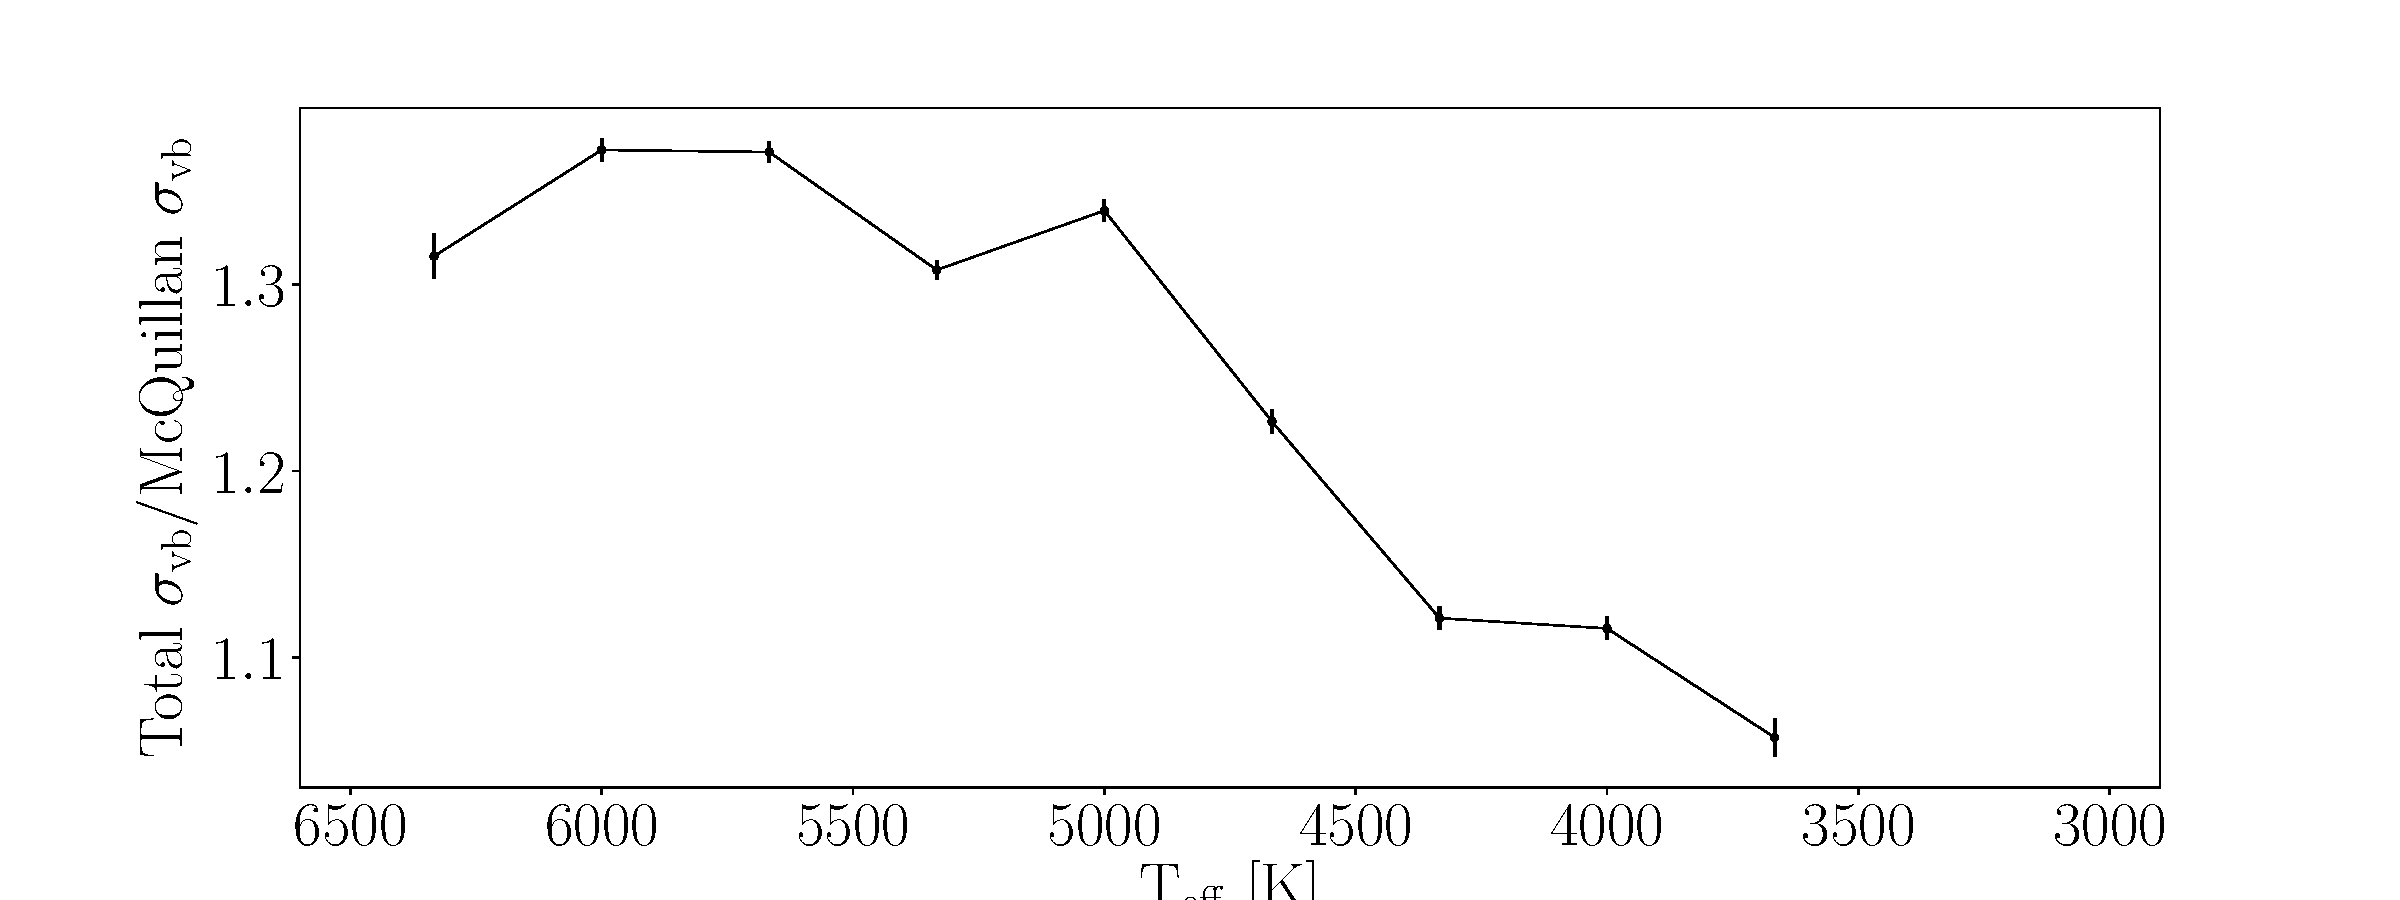
\includegraphics[width=1\textwidth]{field_comparison}
\label{fig:compare}
\end{figure}


\subsection{Synchronized binaries and the \kepler\ period gap}
\label{sec:gap}

\begin{figure}
  \caption{
      Top: rotation period vs. effective temperature for stars in the \mct\
    sample, separated into three groups. Blue circles
      show stars with rotation periods longer than the
    period gap, orange squares show stars with rotation periods shorter than
    the gap, but longer than the lower edge of the main rotation period
    distribution, and green triangles show stars with rotation periods shorter
    than this lower edge.
    Stars were separated into these three groups using \citet{angus2019}
    gyrochronology models, with the scheme shown in the legend.
    Only stars cooler than 5000 K are plotted in
    the bottom panel in order to isolate populations above and below the
    period gap, which only extends up to temperatures of $\sim$4600 K.
    Bottom: the velocities of these groups of stars (in the direction of
    Galactic latitude, $b$) are shown as a function of rotation period.
    The black line indicates the velocity standard deviation as a function of
    period.
}
  \centering
    \includegraphics[width=1\textwidth]{gap}
\label{fig:gap}
\end{figure}

In this section, we explored the kinematic properties of the \mct\ sample in
more detail, investigating the velocity dispersions of stars either side of the
\kepler\ period gap, and identifying rapidly rotating stars that may be
synchronized binaries.

There is a sharp gap in the population of rotation periods (often called the
\kepler\ period gap), which lies just above the 1 Gyr gyrochrone in the upper
panel of figure \ref{fig:vplot}, whose origin is unknown and is the subject of
much speculation \citep{mcquillan2014, davenport2018, reinhold2019}.
This gap was first identified by \mct, and roughly follows a line of constant
gyrochronal age of around 1.1 Gyr \citep[according to the][gyrochronology
relation]{angus2019}.
Several explanations for the gap's origin have been proposed, including a
discontinuous star formation history \citep{mcquillan2013, davenport2017,
davenport2018} and a change in magnetic field structure causing a brief period
where rotational variability is reduced and rotation periods cannot be
measured \citep{reinhold2019}.

The top panel of figure \ref{fig:vplot} suggests that the \citet{angus2019},
Praesepe-based gyrochronology model is valid below the gap but not above.
Gyrochrones follow lines of constant velocity dispersion below the gap, but
{\it cross} lines of constant velocity dispersion above the gap.
This phenomenon is robust to the choice of bin size and position.
Although we do not provide an in-depth analysis here (and more data may be
needed to confirm a connection) these data suggest that the gap may indeed
separate a young regime where stellar cores are decoupled from their envelopes
from an old regime where these layers are more tightly coupled.
If so, this could indicate that the phenomenon responsible for changing the
shape of gyrochrones in rotation-\teff\ space is related to the phenomenon that
produces the gap.

An alternate explanation for the gap is that the \mct\ sample contains two
distinct stellar populations: one young and one old.
If so, the kinematic properties of stars above and below the gap are likely to
be distinctly different.
The bottom panel of figure \ref{fig:gap} shows the velocity dispersions of
stars in the \mct\ sample, with stars subdivided into three groups: those that
rotate more quickly than the main rotation period population (green
triangles), those with rotation periods shorter than the gap (orange squares),
and those with rotation periods longer than the gap (blue circles).
Stars were separated into these three groups using \citet{angus2019}
gyrochronology model, according to the scheme shown in the legend.
Only stars cooler than 5000 K are included in the bottom panel in order to
isolate populations above and below the period gap, which only extends up to a
temperature of $\sim$4600 K in our sample \citep[Although][found that the gap
extends to temperatures as hot as 6000 K]{davenport2017}.
In general, velocity dispersion increases with rotation period because both
quantities increase with age.
There is a smooth transition in velocity dispersion between stars with
rotation periods below and above the gap (orange squares to blue circles),
suggesting that these groups are part of the same Galactic population.
Previously, only the overall velocity dispersions of all stars above and below
the gap have been compared, leading to the assumption that these groups belong
to two distinct populations \citep{mcquillan2014}.
The smooth increase in velocity dispersion across the gap shown here suggests
that stars above and below are part of the same stellar population.
However, it does not rule out the possibility that a brief cessation of star
formation in the Solar neighborhood, around one Gyr ago, may have caused this
gap.

In the final part of our analysis, we investigated the potential for using
kinematics to identify synchronized binaries in the \mct\ sample.
Synchronized binaries are pairs of stars whose rotation periods are equal to
their orbital period.
Since synchronization appears to happen at rotation periods of 7 days or
shorter \citep{simonian2019}, and most isolated stars have rotation periods
longer than 7 days, the rotation periods of synchronized binaries are likely
to be {\it shorter} than they would be if they were isolated stars.
For this reason, their rotation periods do not reflect their ages and the
gyrochronal age of a synchronized binary is likely to be much younger than the
true age of the system.
Synchronized binaries are therefore a source of contamination for
gyrochronology and should be removed from samples before performing a
gyrochronal age analysis.
Figure \ref{fig:gap} shows that some of the most rapidly rotating stars in the
\mct\ sample have relatively large absolute velocities, indicating that they
are likely synchronized binaries.
For this reason, the velocity dispersions of stars with rotation periods
shorter than the lower edge of the rotation period distribution (green
triangles in figure \ref{fig:gap}) are not significantly smaller than the,
presumed older, orange-colored stars.
In general, stars with rotation periods less than $\sim$10 days have an
increased chance of being synchronized binaries.
This result is in agreement with a recent study which found that a large
fraction of photometric binaries were rapid rotators, and the probability of a
star being a synchronized binary system substantially increased below rotation
periods of around 7 days \citep{simonian2019}.
We caution users of rotation period catalogs that rapid rotators with large
absolute velocities should be flagged as potential synchronized binaries
before applying any gyrochronal analysis.


% % Word limit: 500
% \section{Discussion}
\label{sec:discussion}

\subsection{The period gap}
\label{sec:period_gap}

The origin of the rotation period gap, first identified
by \citet{mcquillan2013} and visible in figures \ref{fig:age_cut} and
\ref{fig:dispersion_period_teff} still remains a mystery.
This gap can be seen as an under-density of points between the 0.7-1.0 and
1.0-1.5 Gyr age ranges in figure \ref{fig:age_cut} and roughly follows a line
of constant gyrochronal age of around 1.1 Gyr \citep[according to the
gyrochronology relation of][]{angus2019}, as shown in figure
\ref{fig:dispersion_period_teff}.
Several explanations for the gap's origin have been proposed, including a
discontinuous star formation history \citep{mcquillan2013, davenport2017,
davenport2018}, a rapid change in magnetic field structure
\citep{reinhold2019}, and erroneous rotation period measurements that are
incorrect by a factor of two \citep{koen2018}.
The latter explanation can be ruled out because stars below the gap have
smaller velocity dispersions than the stars above the gap, indicating that
they are kinematically younger \citep{mcquillan2013, davenport2018}, as
evident in figures \ref{fig:age_cut} and \ref{fig:dispersion_period_teff}.

For stars below the gap, in the 0.7-1.0 Gyr age range shown in figure
\ref{fig:age_cut}, velocity dispersion is relatively constant as a function of
temperature, however above the gap, in the 1.0-1.5 Gyr age range and older,
velocity dispersion increases with \teff.
The coolest stars in the 1.0-1.5 Gyr age range have the same velocity
dispersion as the mid-temperature stars in the age range above, and the
hottest stars in the age range above {\it that}, which indicates that the
period-\teff\ relations are {\it flat} at rotation periods between $sim$15-25
days, for 5500 K $<$ \teff\ $<$ 4000 K.
Below the gap, velocity dispersion within a given period range appears to {\it
decrease} with decreasing temperature.
The opposite appears to be true above the gap.

The gap may be positioned at a significant Rossby number/age at which stellar
magnetic dynamos go through a transition.
Perhaps before the age of 1.1 Gyr, or at Rossby numbers less than ???,
magnetic braking is more efficient for stars with deeper convection zones.
Once stars reach this critical age or Rossby number their magnetic fields
undergo some transition, which produces the gap in the rotation period-\teff\
plane and after this transition, magnetic braking efficiency no longer
increases with decreasing mass.
Of course, it may be a coincidence that the gyrochronology relations seem to
only flatten off above the period gap and we lack a sufficient quantity of
data to do more than speculate here.
New rotation periods from the \ktwo\ and \tess\ missions may be able to
validate or rule out this hypothesis in the future.

In the $\sim$ 1.1 Gyr NGC 6811 cluster, the rotation periods of mid-K dwarfs
are faster than expected; their rotational evolution appears to have stalled,
and they have similar rotation periods to the 650 Myr Praesepe cluster
\citep{curtis2019}.
The rotation periods of the K dwarfs in NGC 6811 are plotted in figure
\ref{fig:dispersion_period_teff}.
Although NGC 6811's G dwarfs fall on the 1.1 Gyr gyrochronology model, the K
dwarfs lie only a little above the 0.65 Gyr gyrochronology model.
NGC 6811 straddles the rotation period gap: its G dwarfs lie above it and its
K dwarfs lie below it.
This cluster may be the `missing link' that connects two epoch of stellar
spin-down.
However, figure \ref{fig:age_cut} indicates that the Praesepe gyrochronology
model is, on average, a {\it good} model for stars younger than $\sim$1 Gyr
% and this model has a very different shape to the NGC 6811 cluster.
suggesting that stars in the field follow the period-color/\teff\ relation of
Praesepe, at least up to around 1 Gyr.
We do not see strong evidence of K dwarf stalling in the field.
% , however without more observations of middle-aged open clusters it : an
% early stage where the period-\teff\ relation for cool dwarfs has a negative
% slope and a late stage where it has a positive slope.
% In this case the period gap may delineate the transition between these two
% regimes and is the point at which stellar magnetic dynamos likely undergo a
% dramatic structural shift at an age of $\sim$ 1.1 Gyr.

% \subsection{Caveats}
% \label{sec:caveats}

% There are some alternative explanations for the trends seen in figures
% \ref{fig:age_cut} and \ref{fig:}
% We list these potential issues below.
% \begin{itemize}
% \item{
% The selection function for these data is extremely complicated, etc.
% }
% \item{
% Redenning for the coolest stars.
% }
% \item{
% Planets/companions for the coolest stars.
% }
% \item{
% Subgiant contamination/weakened magnetic braking.
% }
% \end{itemize}


% Word limit: 250
\section{Conclusion}

In this paper, we demonstrated that the dispersion of velocities in the
direction of galactic latitude, \vb, can be used as an age proxy, by showing
that there is no strong evidence for mass-dependent heating in low-mass
\kepler\ dwarfs: the velocity dispersions of K and M dwarfs, whose
main-sequence lifetimes are longer than around 11 Gyrs, do not appear to
increase with decreasing mass.
Although {\it vertical} velocity, \vz, is a quantity that has been
demonstrated to trace time-dependent orbital heating in the disc of the
Galaxy, most stars with measured rotation periods do not yet have radial
velocities, so we used velocity in the direction of Galactic latitude, \vb\,
as a proxy for \vz.
Using stars in the GUMS simulation, we showed that using \vb\ as a proxy for
\vz\ introduces an additional velocity dispersion, which increases with
increasing Galactic latitude.
For this reason we did not attempt to convert \vb\ dispersions into ages using
an age-velocity dispersion relation.
However, after removing high-latitude ($b>15^\circ$) stars from the sample, we
confirmed that using \vb\ instead of \vz\ does not introduce any
mass-dependent velocity dispersion bias into the sample.
We therefore assumed that \vb\ velocity dispersion can be used to accurately
rank stars by age, \ie\ a group of stars with a large velocity dispersion is,
on average, older than a group of stars with a small velocity dispersion.

% We found that old groups of cool dwarfs, selected to be coeval using the
% \citet{angus2019} gyrochronology relation, do {\it not} have the same velocity
% dispersion across all temperatures.
We used the \vb\ velocity dispersions of stars in the \mct\ catalog to explore
the evolution of stellar rotation period as a function of effective
temperature and age.
We found that the \citet{angus2019} relation, which is based on the
period-color relation of the 650 Myr Praesepe cluster, does not correctly
describe the period-age-\teff\ relation for old stars.
Instead we found that, at young ages, rotation period is anti-correlated with
\teff: cooler stars spin more slowly than hotter stars of the same age.
However, at intermediate ages the relation flattens out and K dwarfs rotate at
the same rate, regardless of mass.
At old ages, it seems that cooler K dwarfs spin more rapidly than hotter K
dwarfs of the same age.
We showed that the period-\teff\ relations change shape over time in a way
that qualitatively agrees with theoretical models which include a
mass-dependent core-envelope angular momentum transport \citep{spada2019}.

% The period-color/\teff\ relation seems to start flattening out after $\sim$1
% Gyr (see figure \ref{fig:age_cut}), potentially around the same age, or just
% older than the period gap which is located at a gyrochronal age of around
% $\sim$1.1 Gyr (see figure \ref{fig:dispersion_period_teff}).
We also found that the oldest stars in the \mct\ catalog are cooler than 4500
K, which suggests that lower-mass stars remain active for longer, allowing
their rotation periods to be measured at older ages.
We speculate that the rotation period gap \citep{mcquillan2014} may separate
a young regime where stellar rotation periods decrease with increasing mass
from an old regime where periods increase with increasing mass, however more
data are needed to provide a conclusive result.
The velocity dispersions of stars increase smoothly across the rotation period
gap, indicating that the gap does not separate two distinct populations.
Finally, we used kinematics to indicate that there is a population of
synchronized binaries with rotation periods less than around 10 days.

% We outlined a number of scenarios which could provide alternative
% explanations for these observations, including incorrect dust corrections for
% the lowest-mass stars and an excess of companions increasing the velocity
% dispersion for these stars.

% If the period-color/\teff\ relation does invert at old ages as our results
% suggest, this would be a paradigm shift for gyrochronology.
% Stellar spin-down rate is thought to be directly tied to magnetic field
% strength, and the deeper convection zones of cooler stars generate stronger
% magnetic fields which {\it should} lead to more efficient angular momentum
% loss.
% However, the micro- and macro-physics of stellar structure and evolution and
% magnetic dynamo models are extremely complicated and a lot is still unknown
% about the magnetic behavior of stars.
% Observations like these can provide useful constraints for physical models,
% and may help to reveal new physical processes at work in stars like our own
% Sun and other planet hosts.


This work was partly developed at the 2019 KITP conference `Better stars,
better planets'.
Parts of this project are based on ideas explored at the Gaia sprints at the
Flatiron Institute in New York City, 2016 and MPIA, Heidelberg, 2017.

This work made use of the gaia-kepler.fun crossmatch database created by Megan
Bedell.

Some of the data presented in this paper were obtained from the Mikulski
Archive for Space Telescopes (MAST).
STScI is operated by the Association of Universities for Research in
Astronomy, Inc., under NASA contract NAS5-26555.
Support for MAST for non-HST data is provided by the NASA Office of Space
Science via grant NNX09AF08G and by other grants and contracts.
This paper includes data collected by the Kepler mission. Funding for the
\Kepler\ mission is provided by the NASA Science Mission directorate.

This work has made use of data from the European Space Agency (ESA) mission
{\it Gaia} (\url{https://www.cosmos.esa.int/gaia}), processed by the {\it
Gaia} Data Processing and Analysis Consortium (DPAC,
\url{https://www.cosmos.esa.int/web/gaia/dpac/consortium}).
Funding for the DPAC has been provided by national institutions, in particular
the institutions participating in the {\it Gaia} Multilateral Agreement.


\bibliographystyle{plainnat}
\bibliography{refs.bib}
\end{document}
